%&pdflatex --translate-file=il2-pl
%Wzór dokumentu
%\usepackage{inputenc}[utf8]
%tu zmień marginesy i rozmiar czcionki
    \documentclass[a4paper,12pt]{article}
    \usepackage[margin=2.5cm]{geometry}
    
 %Lepiej tego nie zmieniaj, jak co to dodawaj pakiety
	\usepackage{titlesec}
	\usepackage{titling}
	\usepackage{fancyhdr}
	\usepackage{mdframed}
	\usepackage{graphicx}
	\usepackage{amsmath}
	\usepackage{amsfonts}
	\usepackage{tabularx}
		\usepackage{tikz}
		\usetikzlibrary{arrows}
		\usepackage[section]{placeins}
		\usepackage{rotating}
%inny wygląd
	%\usepackage{tgbonum}
	
	
	%Zmienne, zmień je!
	\graphicspath{ {./images/} }
	\title{Badanie zależności okresu drgań wahadła od jego długości.}
    \author{Grzegorz Koperwas}
	\date{\today{}}
    
  %lokalizacja polska (odkomentuj jak piszesz po polsku)
  
    \usepackage{polski}
    %\usepackage[polish]{babel} 
    \usepackage{indentfirst}
	\usepackage{icomma} 
	
    \brokenpenalty=1000
    \clubpenalty=1000
    \widowpenalty=1000    
 
 %nie odkometowuj wszystkiego, użyj mózgu
    %\renewcommand\thechapter{\arabic{chapter}.}
	\renewcommand\thesection{\arabic{section}.}
	\renewcommand\thesubsection{\arabic{section}.\arabic{subsection}.}
	\renewcommand\thesubsubsection{\arabic{section}.\arabic{subsection}.\arabic{subsubsection}.}

%Makra
    
	\newcommand{\obrazek}[3]{
	\begin{figure}[h]
		\centering
		\includegraphics[scale=#1]{#2}
		\caption{#3}
	\end{figure}
}     
            
    
    \newcommand{\twierdzonko}[1]{
        \begin{center}
        \begin{mdframed}
        #1
        \end{mdframed}          
        \end{center}
    } 
    
    \newcommand{\dwanajeden}[2]{
	\ensuremath \left( \begin{array}{c}
		#1\\
		#2
	\end{array} \right)
}  
      
%Stopka i head (sekcja której nie powinno się zmieniać)
    \pagestyle{fancy}
    \fancyhead{}
    \fancyfoot{}
    
    %Zmieniaj od tego miejsca
	\rfoot{\thepage}
	%\lfoot{Grzegorz Koperwas, \LaTeX note}
	\renewcommand{\headrulewidth}{0pt}
	\renewcommand{\footrulewidth}{1pt}
\titleformat{\section}{\Large \bfseries}{}{1em}{\thesection \hspace{0.5em}}[\titlerule]
    
\begin{document}
\begin{titlepage}
		\maketitle
		\thispagestyle{empty}
\end{titlepage}


\section{Wstęp teoretyczny}

Celem doświadczenia było wyznaczenie przyspieszenia grawitacyjnego $g$ poprzez pomiar czasu
w jakim wahadło wykona 10 cykli w zależności od długości wahadła. 

\begin{figure}[h]
		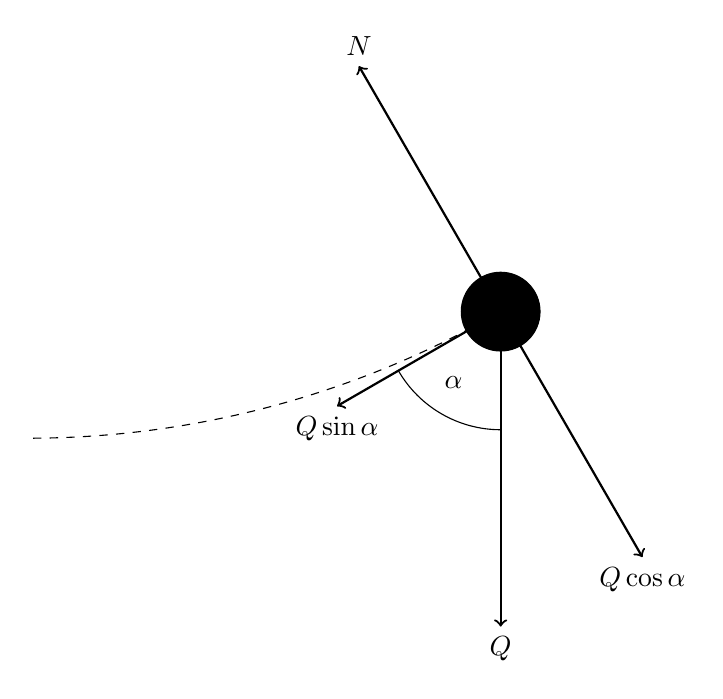
\begin{tikzpicture}[scale = 1]
				\draw [fill = black] (0,0) circle [radius = 0.5];
				\draw [->, thick] (0,0) -- (0, -4) node [below]{$Q$};
				\draw [->, thick, rotate = 30, scale= 0.9] (0,0) -- (0, -4) node [below]{$Q\cos\alpha$};
				\draw [->, thick, rotate = -60, scale= 0.6] (0,0) -- (0, -4) node [below]{$Q\sin\alpha$};
				\draw [->, thick, rotate = 210, scale= 0.9] (0,0) -- (0, -4) node [above]{$N$};
				\draw [rotate = 210, scale = 1.5](1,0) arc (0:60:1);
				\node at (-.6,-.9){$\alpha$};
				\draw [dashed, thin, rotate = -60](0,0) arc (0:-30:12);
		\end{tikzpicture}
		\centering
		% Jak masz to zamiar zajebać mi Kamilu Kowalski (lub ktokolwiek inny) to wiedz że wisisz mi piwo lub 3
		% Jak myślisz że się nie skapnę to jesteś w błędzie
		% Za długo czasu mi zrobienie tego gówna zajeło byś ty kochany człeku se to ukradł
		\caption{Wahadło w stanie największego wychylenia}
\end{figure}

Gdzie:
\begin{itemize}
		\item $Q$ - ciężar
		\item $N$ - naciąg
\end{itemize}

Z praw Newtona:
\[F = ma\]

Gdzie F jest siłą wypadkową działającą na wahadło. Na wahadło działa siła ciężkości i naciągu
sznurka. Siła naciągu jest równa składowej siły ciężkości prostopadłej do toru ruchu wahadła,
zatem siła wypadkowa jest równa równoległej składowej siły ciężkości. Zatem:
\begin{align*}
		ma &= -mg\sin \alpha \\
		a &= -g\sin \alpha
\end{align*}

Przyspieszenie $a$ może zostać powiązane z zmianą kąta $\alpha$. Niech $s$ to długość łuku
zakreślanego przez wahadło.
\begin{align*}
		s &= l\alpha\\
		v &= \frac{ds}{dt} = l \frac{d\alpha}{dt}\\
		a &= \frac{d^2s}{dt^2} = l \frac{d^2 \alpha}{d t^2}
\end{align*}
zatem:
\begin{align*}
		l \frac{d^2 \alpha}{d t^2} &= -g \sin \alpha
\end{align*}
\begin{equation}
		\frac{d^2 \alpha}{d t^2} + \frac{g}{l}\sin \alpha = 0
		\label{eq:preAprox}
\end{equation}

Dla małych kątów możemy założyć że $\sin \alpha\approx \alpha$, zatem po podstawieniu do równania
\ref{eq:preAprox} otrzymujemy równanie oscylatora harmonicznego:
\[ \frac{d^2 \alpha}{d t^2} + \frac{g}{l} \alpha = 0 \]

Dla warunków początkowych $\alpha \left( 0 \right) = \alpha_0$ i $\frac{d\alpha}{dt}\left( 0 \right) = 0$:
\[ \alpha \left( t \right) = \alpha_0 \cos\left(\sqrt{\frac{g}{l}}t \right) \]

Zatem okres jest równy:
\begin{equation}
		T = 2\pi \sqrt{\frac{l}{g}} \qquad \text{dla małych kątów}
		\label{eq:okres}
\end{equation}

Ostatecznie w celu uzyskania wykresu $T^2 \left(l\right)$:
\begin{equation}
		T^2\left( l \right) = \frac{4\pi^2}{g}  \cdot l
		\label{eq:wykres}
\end{equation}

\begin{sidewaystable}[p]
		\centering
		\Large
		\begin{tabular}{|c|c|c|c|c|c|c|c|c|c|c|}
				\hline
	długość             &\multicolumn{10}{c|}{czas t (s) $\pm 0,01$s} \\ \cline{2-11}
	l (cm) $\pm 0,1$cm	& $t_1$ & $t_2$ & $t_3$ & $t_4$ & $t_5$ & $t_6$ & $t_7$ & $t_8$ & $t_9$ & $t_{10}$\\ \hline
		  80,0  & 18,32 & 17,72 & 18,28 & 18,01 & 18,29 & 18,18 & 17,87 & 17,72 & 18,03 & 18,18\\
		  70,0  & 16,66 & 16,73 & 16,84 & 16,93 & 16,67 & 16,67 & 16,83 & 16,91 & 16,68 & 16,67\\
		  60,0  & 15,37 & 15,43 & 15,71 & 15,52 & 15,55 & 15,28 & 15,48 & 15,54 & 15,50 & 15,59\\
		  50,0  & 14,16 & 14,14 & 14,17 & 14,25 & 14,13 & 14,29 & 14,32 & 14,16 & 14,23 & 14,23\\
		  40,0  & 12,77 & 12,55 & 12,61 & 12,54 & 12,86 & 12,68 & 12,64 & 12,72 & 12,61 & 12,63\\
		  30,0  & 11,03 & 10,98 & 10,95 & 10,94 & 10,95 & 10,73 & 10,93 & 11,06 & 10,87 & 10,87\\
		  20,0  & 8,87 & 8,97 & 9,02 & 9,01 & 8,97 & 8,99 & 8,91 & 8,88 & 8,93 & 8,84\\
		  10,0  & 6,09 & 6,27 & 6,18 & 6,20 & 6,25 & 6,49 & 6,18 & 6,33 & 6,25 & 6,27\\\hline
\end{tabular}
		\caption{Tabela wyników pomiarów}
		\label{tab:pomiar}
\end{sidewaystable}

\section{Analiza wyników pomiarów}

Dla wyników doświadczenia w tabeli \ref{tab:pomiar} obliczamy:
\begin{itemize}
		\item Średni czas $\bar{t}$.
		\item Odchylenie standardowe średniego czasu $\Delta \bar{t}$.
		\item Okres wychyleń wahadła $T$.
		\item Niepewność okresu $\Delta T$.
		\item Kwadrat okresu $T^2$.
		\item Niepewność kwadratu okresu $\Delta \left( T^2 \right)$.

\end{itemize}
\subsection*{Odchylenie standardowe}
Odchylenie standardowe średniej jest równe:
\[ \Delta \bar{t} = \sqrt{\frac{\sum \limits^n_{i = 1}\left( x_i - \bar{x}\right)^2}{n\left(n-1 \right)}}\]
Przykładowo:
\begin{align*}
		&\sqrt{\frac{\left( 6,09- 6,25 \right)^2 +
		\left( 6,27- 6,25 \right)^2 +
		\left( 6,33- 6,25 \right)^2 +_{\dots} +
		\left( 6,25- 6,25 \right)^2 +
		\left( 6,27 - 6,25 \right)^2}{10 \cdot 9}} =\\
		&= \sqrt{\frac{0,03 + 0,00 + 0,01 + 0,00 + 0,00 + 0,06 + 0,01 + 0,01 + 0,00 + 0,00}{90}} = \\
		&\approx 0,03
\end{align*}

\subsection*{Okres}

Okres wychyleń wahadła obliczamy za pomocą wzoru:
\[ T = \frac{\bar{x}}{n}\]
gdzie $n$ to liczba wychyleń wykonanych przez wahadło w czasie mierzonym $t$.

Przykładowo:
\[ \frac{18,06}{10} \approx 1,80 \]
Niepewność okresu wychyleń obliczamy w sposób analogiczny.

\subsection*{Kwadrat okresu}

Niepewność $T^2$ jest obliczana w poniższy sposób:
\[\frac{\Delta \left(T^2\right)}{T^2} = \frac{\Delta T}{T} + \frac{\Delta T}{T} = 2 \cdot \frac{\Delta T}{T}\]

\begin{table}[h]
		\centering
		\begin{tabular}{|c|c|c|c|c|c|c|}
				\hline
				długość l (cm) $\pm 0,1$cm & $\bar{t}$ & $\Delta \bar{t}$ & $T$ & $\Delta T$ & $T^2$ & $\Delta \left( T^2 \right)$ \\ \hline 
  80,0  & 18,06 & 0,07 & 1,81 & 0,01 & 3,26 & 0,01\\
  70,0  & 16,76 & 0,03 & 1,68 & 0,00 & 2,81 & 0,01\\
  60,0  & 15,50 & 0,04 & 1,55 & 0,00 & 2,40 & 0,01\\
  50,0  & 14,21 & 0,02 & 1,42 & 0,00 & 2,02 & 0,00\\
  40,0  & 12,66 & 0,03 & 1,27 & 0,00 & 1,60 & 0,01\\
  30,0  & 10,93 & 0,03 & 1,09 & 0,00 & 1,19 & 0,01\\
  20,0  & 8,94 & 0,02 & 0,89 & 0,00 & 0,80 & 0,00\\
  10,0  & 6,25 & 0,03 & 0,63 & 0,00 & 0,39 & 0,01\\\hline 

		\end{tabular}
		\caption{Tabela obrobionych wyników}
		\label{tab:obrobione}
\end{table}

\begin{sidewaysfigure}[p]
		\centering
		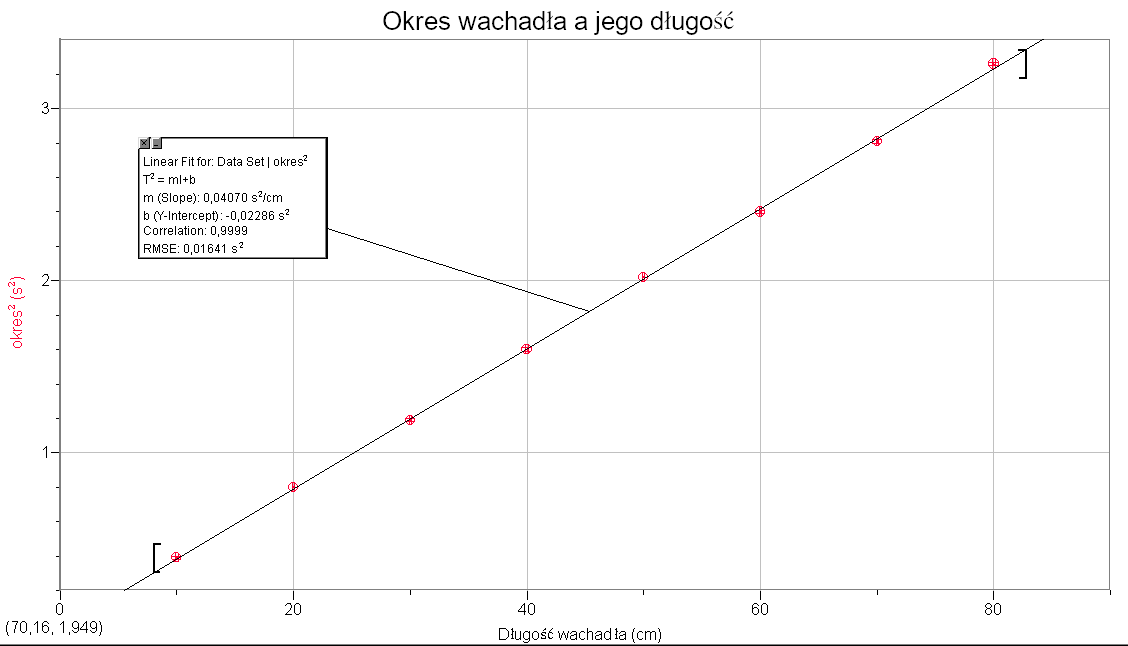
\includegraphics[width = \linewidth]{wykres}
		\caption{Wykres funkcji $T^2 \left( l \right)$}
		\label{fig:wykres}
\end{sidewaysfigure}
\section{Wnioski}
\subsection*{Obliczanie przyspieszenia grawitacyjnego:}

Nachylenie wykresu $m$ funkcji z równania \ref{eq:wykres} jest równe:
\[m = \frac{4\pi^2}{g} \]
zatem:
\begin{align*}
		g &= \frac{4\pi^2}{m}\\
		g &= \frac{4\pi^2}{0,0407 \cdot 10^2} \approx 9,70 \frac{m}{s^2}
\end{align*}
Z programu \emph{Logger Pro} niepewność $m$ wynosi $0,0002532 \, \frac{s^2}{\text{cm}}$ więc ostatecznie:
\[ g \approx \left( 9,70 \pm 0,03 \right) \, \frac{m}{s^2} \]

Dla Gliwic przyspieszenie grawitacyjne wynosi:
\[ g_{\text{std}} = 9,81 \, \frac{m}{s^2}\]
Zatem błąd względny otrzymanej wartości wynosi:
\begin{align*}
		\Delta g &= \frac{\left|g_{\text{std}} - g\right|}{g_{\text{std}}} \cdot 100 \text{\%} \\
		\Delta g &= \frac{| 9,81 - 9,70|}{9,81} \cdot 100 \text{\%} \approx\\
		&\approx 1,12 \text{\%}
\end{align*}

\subsection*{Możliwe źródła niepewności i błędów:}

Na jakość pomiarów głównie wpływał błąd losowy pomiaru czasu oraz błędy losowe i systematyczne pomiaru długości wahadła. Znając
wady używanej przez nas metody czasu postanowiliśmy im przeciwdziałać poprzez dokonywanie dziesięciu pomiarów dla każdej
długości wahadła, patrząc na obliczone przez nas odchylenia standardowe możemy zauważyć że wpływ losowości tej metody na wynik
doświadczenia był pomijalny.

Jednakże nie zostały przez nas podjęte żadne działania mające na celu ograniczenie wpływu błędu systematycznego, który mógł wynikać
z złej metody pomiaru długości sznurka na którym został powieszony ciężarek będący wahadłem. Miarka którą dokonywaliśmy pomiaru była
przymocowana na stałe do statywu, jednak była przesunięta względem punktu do którego było przymocowane wahadło, miarka również
mogła nie być równoległa względem sznurka podczas pomiaru, mógł wystąpić znaczący błąd paralaksy. Być może z tego powodu wykres
oparty na naszych danych nie przechodzi przez początek układu współrzędnych.

W celu poprawy jakości wyników powinniśmy byli dokonywać bezpośredniego pomiaru długości sznurka miarką, która nie była przyczepiona
na stałe do statywu.

Na wynik eksperymentu mógł mieć wpływ również opór powietrza jak i niedoskonałe właściwości sznurka, jednak ich wpływu nie jestem w
stanie określić.
\listoftables
\listoffigures



\end{document}
